%%%%%%%%%%%%%%%%%%%%%%%%%%%%%%%%%%%%%%%%%
% Short Sectioned Assignment
% LaTeX Template
% Version 1.0 (5/5/12)
%
% This template has been downloaded from:
% http://www.LaTeXTemplates.com
%
% Original author:
% Frits Wenneker (http://www.howtotex.com)
%
% License:
% CC BY-NC-SA 3.0 (http://creativecommons.org/licenses/by-nc-sa/3.0/)
%
%%%%%%%%%%%%%%%%%%%%%%%%%%%%%%%%%%%%%%%%%

%----------------------------------------------------------------------------------------
%	PACKAGES AND OTHER DOCUMENT CONFIGURATIONS
%----------------------------------------------------------------------------------------

\documentclass[paper=a4, fontsize=11pt]{scrartcl} % A4 paper and 11pt font size

\usepackage[T1]{fontenc} % Use 8-bit encoding that has 256 glyphs
\usepackage{fourier} % Use the Adobe Utopia font for the document - comment this line to return to the LaTeX default
\usepackage[spanish]{babel} % English language/hyphenation
\selectlanguage{spanish}
\usepackage[utf8]{inputenc}
\usepackage{amsmath,amsfonts,amsthm} % Math packages
\usepackage{graphicx}

\usepackage{sectsty} % Allows customizing section commands
\allsectionsfont{\centering \normalfont\scshape} % Make all sections centered, the default font and small caps

\usepackage{fancyhdr} % Custom headers and footers
\pagestyle{fancyplain} % Makes all pages in the document conform to the custom headers and footers
\date{}
\fancyhead{} % No page header - if you want one, create it in the same way as the footers below
\fancyfoot[L]{} % Empty left footer
\fancyfoot[C]{} % Empty center footer
\fancyfoot[R]{\thepage} % Page numbering for right footer
\renewcommand{\headrulewidth}{0pt} % Remove header underlines
\renewcommand{\footrulewidth}{0pt} % Remove footer underlines
\setlength{\headheight}{5.6pt} % Customize the height of the header

\numberwithin{equation}{section} % Number equations within sections (i.e. 1.1, 1.2, 2.1, 2.2 instead of 1, 2, 3, 4)
\numberwithin{figure}{section} % Number figures within sections (i.e. 1.1, 1.2, 2.1, 2.2 instead of 1, 2, 3, 4)
\numberwithin{table}{section} % Number tables within sections (i.e. 1.1, 1.2, 2.1, 2.2 instead of 1, 2, 3, 4)

\setlength\parindent{0pt} % Removes all indentation from paragraphs - comment this line for an assignment with lots of text

%----------------------------------------------------------------------------------------
%	TITLE SECTION
%----------------------------------------------------------------------------------------

\newcommand{\horrule}[1]{\rule{\linewidth}{#1}} % Create horizontal rule command with 1 argument of height

\title{	
\normalfont \normalsize 
\textsc{UNIVERSIDAD DE CANTABRIA, DEPARTAMENTO DE FÍSICA MODERNA} \\ [20pt] % Your university, school and/or department name(s)
\horrule{0.5pt} \\[0.4cm] % Thin top horizontal rule
\huge Física de Partículas Elementales (G71) \\ % The assignment title
\normalsize 4 Curso - Grado de Física - Primer parcial
\horrule{2pt} \\[0.5cm] % Thick bottom horizontal rule
}

\begin{document}

\maketitle % Print the title

\vspace{-2.5cm}

%----------------------------------------------------------------------------------------
%	PROBLEM 1
%----------------------------------------------------------------------------------------
\textbf{Cuestión 1.} El CERN produce un haz de neutrinos muónicos que es detectado en el experimento OPERA (Grand Saso, Italia). El haz de neutrinos 
se produce a través del decaimiento del pión cargado ($\pi^{+}\rightarrow\mu^{+}+\nu_\mu$). Si la energía de los piones es de 10 GeV y los muones 
que son detectados a un ángulo dado tienen una energía de 6 GeV, ¿Qué ángulo forman los neutrinos con la dirección de los muones?. Considera la masa
de los neutrinos despreciable, y $m(\pi^{+})=0.140$ GeV y $m(\mu^{+})=0.106$ GeV. \textbf{(2 Puntos)}.
\\
\\
%----------------------------------------------------------------------------------------
%       PROBLEM 2
%----------------------------------------------------------------------------------------
\textbf{Cuestión 2.} Define los siguientes conceptos indicando si se trata de magnitudes invariantes bajo transformaciones de Lorentz: tasa de transición,
sección eficaz, densidad de estados, elemento de matriz $T_{if}$.\textbf{(2 Puntos)}.
\\
\\
%----------------------------------------------------------------------------------------
%       PROBLEM 3
%----------------------------------------------------------------------------------------
\textbf{Cuestión 3.} Prueba las siguientes relaciones de las matrices $\gamma$ \textbf{(1 Punto)}: 
\begin{enumerate}
\item $\gamma_\mu\gamma^\mu=4I$
\item $\gamma_\mu\gamma_\nu a^{\nu}\gamma^{\mu}=-2\gamma_\nu a^{\nu}$
\end{enumerate}
%----------------------------------------------------------------------------------------
%       PROBLEM 4
%----------------------------------------------------------------------------------------
\textbf{Cuestión 4.} Demuestra que cada una de las componentes de los espinores de Dirac cumple la ecuación de Klein-Gordon ($\partial_\mu\partial^{\mu} + m^2)\psi_i = 0$. Para ello multiplica a la ecuación de Dirac por $(i\gamma^{\nu}\partial_{\nu} + m)$ y opera sabiendo que $\gamma^{\nu}\gamma^{\mu}a_{\mu}a_{\nu}=\frac{1}{2}(\gamma^{\nu}\gamma^{\mu} + \gamma^{\mu}\gamma^{\nu})a_{\mu}a_{\nu}$. \textbf{(1 Punto)}.
%----------------------------------------------------------------------------------------
\\
\\
%----------------------------------------------------------------------------------------
%       PROBLEM 5
%----------------------------------------------------------------------------------------
\textbf{Cuestión 5.} Definir el concepto de helicidad. ¿Por qué se dice que el momento angular orbital no es una buena magnitud para estudiar las soluciones de la ecuación de Dirac? \textbf{(1 Punto)}.
\\
\\
%----------------------------------------------------------------------------------------
%       PROBLEM 6
%----------------------------------------------------------------------------------------
\textbf{Cuestión 6.} ¿A qué llamamos operador conjugación de carga y cómo se relaciona con la interacción electromagnética?. Demuestra que si aplicamos el operador conjugación de carga
a los espinores de partícula en \ref{espinores}, obtenemos los espinores de antipartícula. \textbf{(1 Punto)}.
\\
\\
%----------------------------------------------------------------------------------------
%       PROBLEM 7
%----------------------------------------------------------------------------------------
\textbf{Cuestión 7.} Usando el espinor para una partícula de helicidad negativa, demuestra que su cuadricorriente de probabilidad asociada es $j^{\mu}=2p$. Para ello ayúdate de las matrices de Dirac (\ref{matrices}) y recuerda que la normalización de los spinores viene dada por $N=\sqrt{E+m}$. \textbf{(2 Puntos)}.



  

\begin{figure}[!h]
\begin{center}
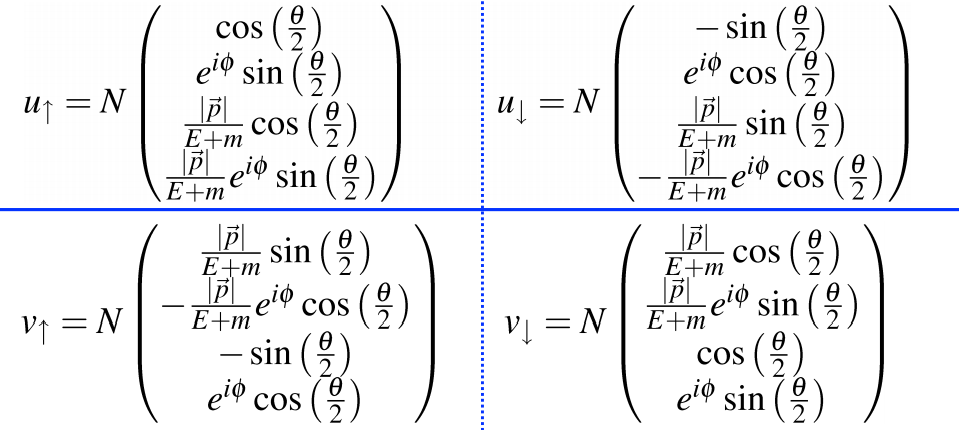
\includegraphics[width=0.6\linewidth]{espinores.png}
\end{center}
\caption{Espinores solución a la ecuación de Dirac y autoestados del operador helicidad.}
\label{espinores}
\end{figure}


\begin{figure}[!h]
\begin{center}
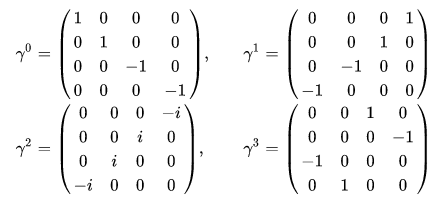
\includegraphics[width=0.6\linewidth]{matrices.png}
\end{center}
\caption{Matrices de Dirac.}
\label{matrices}
\end{figure}






\end{document}
